
\subsection{Contrôle des contacteurs}

	\paragraph*{}
	Pour amener la batterie dans un état sécuritaire, il faut pouvoir la débrancher de l'alimentation. Le système utilise donc des contacteurs à haute puissance pour contrôler la connexion de la batterie avec le reste des charges. Le module maître se charge de contrôler ces contacteurs. Il s'occupe d'enclencher les contacteurs lors de la mise en marche du système lorsqu'aucune faute n'est détectée. De plus, lorsque le module maître reçoit un message d'erreur, il doit s'assurer de déconnecter la batterie pour protéger les modules en cas de fautes.

	\paragraph*{}
	Le système est composé de trois contacteurs, soient deux contacteurs principaux et un pour les MPPTs. L'un des contacteurs principaux est connecté à la borne positive de la batterie et l'autre à la borne négative. On peut voir à la figure suivante un schéma général de la disposition des contacteurs. 
	
	\begin{figure}[H]
		\centering
		\fbox{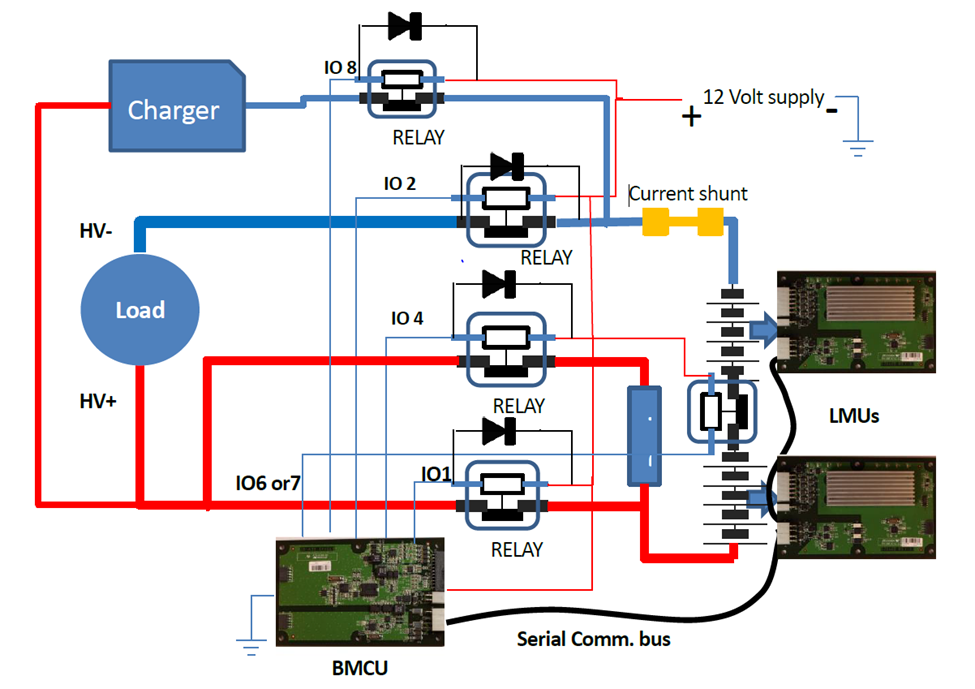
\includegraphics[width=0.6\linewidth]{Images/LithiumBalanceContactorDiagram}}
		\caption[Diagramme général des contacteurs]{Image tirée du guide utilisateur du BMS de LithiumBalance \cite{Lithium_Balance}}
		\label{fig:lithiumbalancecontactordiagram}
	\end{figure}

	\paragraph*{}
	L'enclenchement des contacteurs se fait avec une tension de 12V, qui doit être appliquée à ses bornes. Puisque c'est le microcontrôleur qui envoie la commande d'ouverture ou de fermeture, il doit y avoir une interface de protection entre le 12V aux bornes du contacteur et le 3.3V de la patte GPIO. De façon générale, il n'est pas conseillé d'utiliser des actionneurs mécaniques, tel qu'un relais, pour activer les contacteurs puisqu'ils sont souvent victimes de défaille. 	 

	\subsubsection*{Choix des contacteurs:}
		\paragraph*{}
		Une commandite d'Autobus Lion a permis au club Éclipse de se procurer trois contacteurs de marque GIGAVAC\_HX21. Il faut donc que le module maître puisse interfacer ces contacteurs. Le système de batterie d'Éclipse 9 utilise des contacteurs EV200 et ceux-ci seront utilisés comme pièce de remplacement. La conception du circuit de contrôle doit être compatible avec les deux modèles.

		\paragraph*{}
		Les spécifications des contacteurs Gigavac montrent que le courant consommé lors de l'ouverture de l'inductance est de 4.3 A. En ajoutant une marge de protection d'un facteur de 1.2, les composantes doivent soutenir un courant de jusqu'à 5.16 A pendant 75 ms\cite{GigavacHX21}. 

		\paragraph*{}
		De plus, ce modèle de contacteur possède un deuxième relais interne qui pour faire de l'interverrouillage (interlock), beaucoup utilisé dans le domaine des véhicules. Dans le cas du présent système, ce relais sera utilisé pour activer un témoin lumineux afin d'avertir l'utilisateur de l'état des contacteurs. Avec les contacteurs EV-200, il faudra court-circuiter deux positions sur le connecteur allant sur le module maître pour activer les témoins lumineux.

		\paragraph*{}
		Également, le circuit de contrôle doit répondre aux critères suivants afin d'être jugé sécuritaire\cite{System_Approach}. 

		\begin{itemize}
			\item Prévenir les défaillances qui causent les contacteurs à ouvrir alors qu'ils devraient être fermés
			\item Prévenir les défaillances qui causent les contacteurs à fermer alors qu'ils devraient être ouverts
			\item Prévenir les défaillances qui causent une connexion de la batteries à travers une charge capacitive	
		\end{itemize}


	\subsubsection*{Choix du circuit de contrôle:}
		\paragraph*{}
		Plusieurs solutions ont été évaluées pour contrôler les contacteurs. Parce que cette section est très critique et qu'il ne faut absolument pas que durant la compétition, une défaillance met en panne la voiture solaire. C'est pourquoi le budget n'est pas un critère de sélection mais, plutôt une solution qui est le plus sécuritaire possible.

		\paragraph*{Solution 1: Contrôle par optocoupleurs}
			
		Puisque les activateurs ne doivent pas être de nature mécanique. On peut utiliser des optocoupleurs (Solid State Relays) puisqu'ils sont isolés mécaniquement. Le microcontrôleur doit seulement alimenter une DEL de l'optocoupleur pour l'enclencher. Aussi, dans l'éventualité que le microcontrôleur ait une défaillance, l'optocoupleur s'ouvrira, empêchant ainsi le contacteur de rester fermé. Il faut par contre choisir un optocoupleur capable d'accepter jusqu'à 5.16 A, ce qui limite beaucoup le choix de composantes.
		
		\begin{table}[H]
			\centering
			\caption{Comparaison des optocoupleurs}
			\label{ComparaisonOpto}
			\begin{tabular}{|p{3cm}|p{3cm}|p{3cm}|p{3cm}|}
				\hline
				\textbf{Optocoupleurs} & \textbf{Courant} & \textbf{Résistance} & \textbf{Prix}
				\\ \hhline{|=|=|=|=|}
				CPC1907B & 6 A & 60 mOhm & 9.01 \$ \\ \hline
				CPC1709J & 10 A & 50 mOhm & 10.00 \$ \\ \hline
				CPC1918J & 5.25 A &	100 mOhm & 14.83 \$	\\ \hline
			\end{tabular}
		\end{table}
		
		Le prix de ces composantes est similaire et leur courant de charge est assez robuste. Le choix s'est donc faite sur le CPC17907B en raison de son profil plat qui était plus avantageux avec le placement des pièces sur le module maître.
		
		\begin{figure}[H]
			\centering
			\fbox{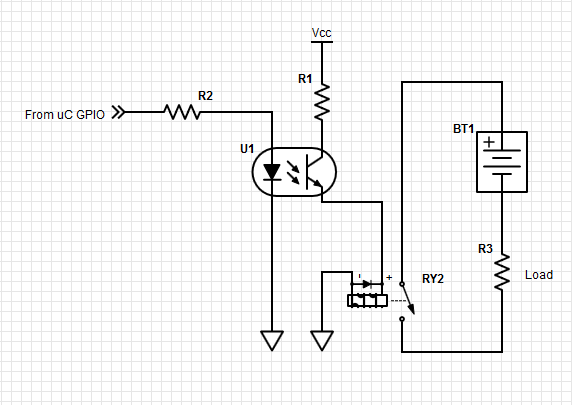
\includegraphics[width=0.4\linewidth]{../Images/ContactorSol1}}
			\caption[]{Schéma Solution 1: Contrôle par optocoupleurs}
			\label{fig:contactorsol1}
		\end{figure}
		
		
		\paragraph*{Solution 2: Contrôle par Mosfet en série}
		\paragraph*{}
		Une façon d'assurer la protection d'un circuit est de rajouter de la redondance. Plusieurs Mosfet sont mises en série pour augmenter les chances d'ouverture de circuit en cas de défaillances. Plus il y a de composantes en série, meilleures sont les chances, mais on augmente aussi le prix en composantes. Chaque Mosfet doit être contrôlé individuellement par une patte du microcontrôleur. Aussi, il est important de s'assurer que la résistance interne des Mosfets soit constante d'une composante à l'autre. C'est pour éviter l'échauffement du Mosfet ayant la résistance interne la plus élevée, pouvant causer des défaillances.
		
		\begin{figure}[H]
			\centering
			\fbox{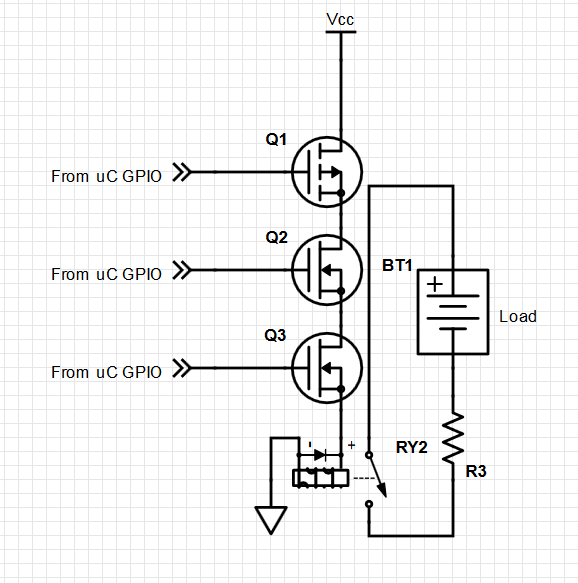
\includegraphics[width=0.4\linewidth]{../Images/ContactorSol2}}
			\caption{Schéma Solution 2: Contrôle par Mosfet en série}
			\label{fig:contactorsol2}
		\end{figure}
		

		\paragraph*{Solution 3: Circuit d'alimentation à double actionneurs}
		\paragraph*{}
		Cette solution provient du livre A systems approach to Lithium-Ion Battery Management \cite{System_Approach}. L'auteur propose d'utiliser circuit d'alimentation à doubles actionneurs, soit un actionneur sur le pôle négatif et un sur le pôle positif. Un Mosfet de type-P alimente le côté positif (High-side) et un mosfet de type-N est ferme le circuit du côté négatif (low-side) ce qui offre une sécurité supplémentaire si une des deux composantes venait à faillir. Puisqu'il y a trois contacteurs dans le système, cette solution requiert d'utiliser un seul Mosfet type-P pour alimenter le côté positif des contacteurs et trois Mosfet type-N pour le côté négatif de chaque relais.

		\begin{figure}[H]
			\centering
			\fbox{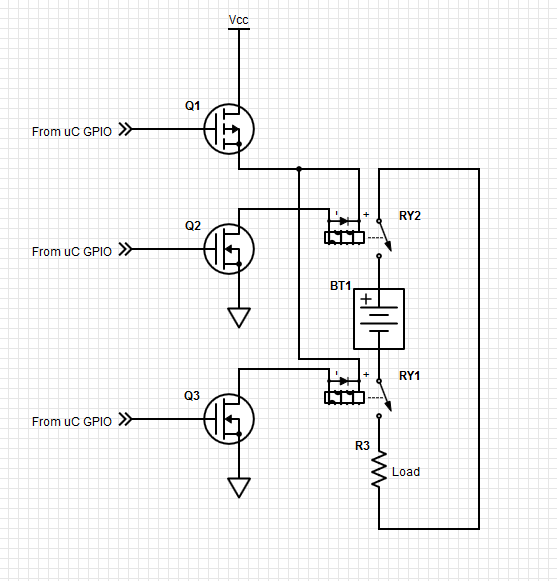
\includegraphics[width=0.4\linewidth]{../Images/ContactorSol3}}
			\caption{Schéma solution 3: Circuit d'alimentation à doubles actionneurs}
			\label{fig:contactorsol3}
		\end{figure}
		
		\paragraph*{Choix final}
		\paragraph*{}
		La solution retenue est un mélange de la solution 1 et 3. En ayant un circuit d'alimentation à doubles actionneurs, on évite d'avoir de la redondance. On remplace ainsi les mosfets de cette solution par les optpocoupleurs de la solution 1. De cette façon, on s'assure de la plus haute protection tout en ayant le minimum de composantes. Puis, puisqu'on veut éviter de tirer trop de courant du microcontrôleur, on utilise un transistor BJT s'activant avec un faible courant. Le BJT peut ensuite alimenter l'optocoupleur avec l'alimentation 3.3V directement.

		\begin{figure}[H]
			\centering
			\fbox{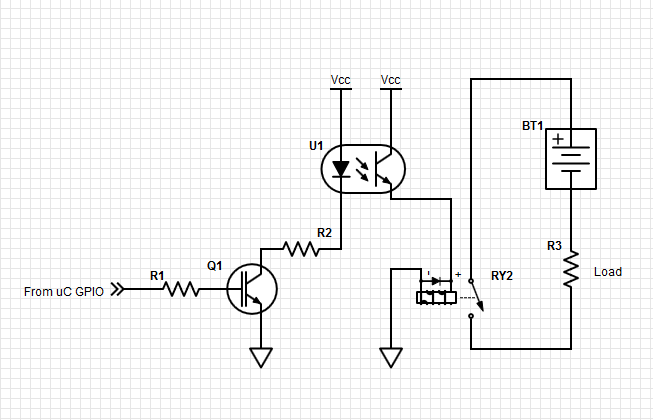
\includegraphics[width=0.4\linewidth]{../Images/ContactorSolFinal}}
			\caption{Choix final}
			\label{fig:contactorsolfinal}
		\end{figure}

	\subsubsection*{Circuit de précharge:}
		\paragraph*{}
		Le contacteur du MPPT et le contacteur principal sur le pôle positif de la batterie possèdent un circuit de précharge. La précharge permet à la batterie de se connecter à une large charge capacitive. Si la batterie est connectée directement avec une charge capacitive déchargée, le courant transitoire sera limité par l'impédance interne de la batterie, de la charge et des contacteurs. Cette limite ne sera généralement pas assez pour prévenir un courant potentiellement dangereux. Un contacteur qui s'enclenche lorsque la différence de potentiel est trop élevée pourrait le souder et empêcher son ouverture\cite{System_Approach}.
		
		\paragraph*{}
		Pour prévenir ce problème, on ajoute une résistance en série avec un relais, installés en parallèle du contacteur. Avant d'enclencher le contacteur, un courant limité passe par la résistance, et permet à la tension de monter de façon exponentielle. On compare ensuite la lecture de la charge avec la tension des batteries. Lorsque la tension sur la charge est assez élevée et que la différence de potentiel aux bornes du contacteur est négligeable, le contacteur peut être fermé de façon sécuritaire\cite{System_Approach}.
		
		\paragraph*{}		
		La résistance de précharge est dimensionnée pour dissiper la puissance circulant dans la résistance. Pour trouver cette valeur, il faut d'abord calculer la constante de temps.
	
		\begin{align}
			\tau =R \cdot C
			\label{eq:Constante de temps}
		\end{align}
				
		On considère la charge capacitive complète après	
	 
		\begin{align}
			T = 5 \cdot \tau
			\label{eq:CapaciteCharge}
		\end{align}
		
		Par mesure de sécurité, on ajoute 0.5 seconde à ce chiffre.
		
		\begin{align}
			T = T + 0.5
			\label{eq:Tempsdecharge}
		\end{align}		
				
		On calcul ensuite l'énergie dissipée par la résistance de précharge.
		
		\begin{align}
			E = \dfrac{C \cdot V^2}{2}
			\label{eq:EnergiePrecharge}
		\end{align}
		
		On trouve finalement la puissance totale consommée par la résistance de précharge
	
		\begin{align}
			P = \dfrac{E}{T}
			\label{eq:PuissancePrecharge}
		\end{align}	
			
		\paragraph*{}		
		Le temps de précharge doit être judicieusement choisi pour s'assurer que la charge capacitive est assez chargée. D'après ces calculs, avec une résistance de 100 Ohm, une durée de 5.5 secondes sera nécessaire si l'on estime la charge capacitive est de 10000uF avec une tension maximale de 160V. 
				
		\begin{table}[H]
			\centering
			\caption{Sélection de la résistances de précharge}
			\label{ResistancePrecharge}
			\begin{tabular}{|p{3cm}|p{5cm}|p{2cm}|p{2cm}|p{1.5cm}|}
				\hline
				\textbf{Composante} & \textbf{Manufacturier} & \textbf{Resistance} & \textbf{Pdissipation} & \textbf{Prix}
				\\ \hhline{|=|=|=|=|=|}
				TR50JBC100R & Stackpole Electronics Inc. & 100 Ohm & 50 W & 5.81 \$ \\ \hline		
			\end{tabular}
		\end{table}

		\paragraph*{}
		Même si la résistance devrait pouvoir soutenir la chaleur, il est possible d'ajouter un dissipateur de chaleur. La résistance ne dissipe qu'une dizaine de watts lorsqu'elle est utilisée seule, comparé à 50W avec un dissipateur.
				
		\begin{table}[H]
			\centering
			\caption{Sélection du dissipateur de chaleur}
			\label{DissipateurPrecharge}
			\begin{tabular}{|p{3cm}|p{4cm}|p{2cm}|p{1.5cm}|}
				\hline
				\textbf{Composante} & \textbf{Manufacturier} & \textbf{Modèle} & \textbf{Prix}
				\\ \hhline{|=|=|=|=|}
				534202B03453G  & Aavid Thermalloy & TO-220 & 1.36 \$ \\ \hline	
				115300F00000G & Aavid Thermalloy & TO-247 & 0.28 \$ \\ \hline	
			\end{tabular}
		\end{table}		 


		\paragraph*{}		
		Le relais doit supporter un courant de 1.6 A. Sa bobine devrait également consommer le moins possible. Un relais tout usage à été choisi.
		
		\begin{table}[H]
			\centering
			\caption{Sélection du relais}
			\label{RelaisPrecharge}
			\begin{tabular}{|p{3cm}|p{3cm}|p{3cm}|p{3cm}|p{3cm}|}
				\hline
				\textbf{Composante} & \textbf{Manufacturier} &  \textbf{Courant} & \textbf{Consommation} & \textbf{Prix}
				\\ \hhline{|=|=|=|=|=|}
				ALQ312 & Panasonic & 10A & 16.7 mA & 3.34 \$ \\ \hline		
			\end{tabular}
		\end{table}				
		
	
		\paragraph*{}	
		Pour éviter de polariser à l'inverse les contacteurs avec la précharge, une diode est ajoutée au circuit. Elle doit bloquer une tension minimum de 160 V et pouvoir supporter un courant d'au moins 1.6 A. 
		
		\begin{table}[H]
			\centering
			\caption{Sélection de la diode}
			\label{DiodePrecharge}
			\begin{tabular}{|p{3cm}|p{3cm}|p{3cm}|p{3cm}|p{3cm}|p{3cm}|}
				\hline
				\textbf{Composante} & \textbf{Manufacturier} & \textbf{Courant} &  \textbf{Baisse de tension} & \textbf{Prix}
				\\ \hhline{|=|=|=|=|=|=|}
				NRVBS3200T3G & ON Semiconductor & 3A & 840 mV @ 3A & 1.37 \$ \\ \hline		
			\end{tabular}
		\end{table}				
		
		\paragraph*{}			
		Ensuite, pour éviter qu'un courant trop élevé ne vienne endommager les composantes, on ajoute un fusible de 2A à action retardée. 
		
		\paragraph*{}			
		La topologie générale du circuit de précharge est présenté à la figure \ref{fig:circuitprecharge}.
				
		\begin{figure}[H]
			\centering
			\fbox{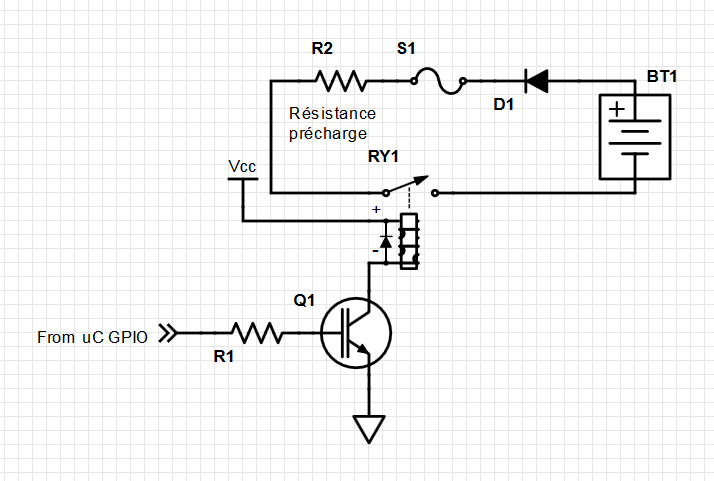
\includegraphics[width=0.7\linewidth]{Images/CircuitPrecharge}}
			\caption[]{Schéma du circuit de précharge}
			\label{fig:circuitprecharge}
		\end{figure}
			
		